\documentclass[10pt,a4paper,oneside,openany]{book}
\usepackage[T1]{fontenc}
\usepackage{lmodern,microtype}
\usepackage[margin=23mm,headheight=14pt]{geometry}
\usepackage{amsmath,amssymb}
\usepackage{graphicx,booktabs,tabularx,caption}
\usepackage{xcolor,fancyhdr}
\usepackage[colorlinks=true,allcolors=reportblue]{hyperref}
\usepackage{subcaption}

\definecolor{reportblue}{HTML}{174B72}
\hypersetup{pdftitle={Discovery and Refinement in Multimodal Black-Box Optimisation},
  pdfauthor={Kwan Li Hao, Beckham Wee Kai Le, Brian Bong Neng Ye }}
\graphicspath{{figures/}}
\renewcommand{\thesection}{\arabic{section}}
\renewcommand{\thefigure}{\arabic{figure}}
\renewcommand{\thetable}{\arabic{table}}
\setcounter{secnumdepth}{2}
\captionsetup{font=small,labelfont=bf}
\setlength{\emergencystretch}{2em}
\setlength{\parindent}{1.25em}
\setlength{\parskip}{0pt}
\setlength{\textfloatsep}{13pt plus 3pt minus 2pt}
\setlength{\intextsep}{11pt plus 3pt minus 2pt}
\renewcommand{\topfraction}{.8}
\renewcommand{\textfraction}{.12}
\linespread{1.02}
\pagestyle{fancy}
\fancyhf{}
\fancyhead[L]{\small DSA4212 Group 1}
\fancyhead[R]{\small Multimodal black-box optimisation}
\fancyfoot[C]{\small\thepage}
\renewcommand{\headrulewidth}{0.35pt}
\raggedbottom
\newcommand{\R}{\mathbb R}
\newcommand{\EI}{\operatorname{EI}}
\newcommand{\sd}{\sigma_0}
\newcommand{\repotree}{https://github.com/bbny27/DSA4212-G1/tree/e2863a9c4a7d237938771be24634e8711d109616}

\begin{document}
\thispagestyle{plain}
\noindent National University of Singapore \hfill DSA4212 \par
\noindent Final Project Report \hfill Group 1\par
\vspace{1.1em}
\begin{center}
{\LARGE\bfseries Discovery and Refinement in\\[0.2em]
Multimodal Black-Box Optimisation\par}
\vspace{0.55em}
\vspace{0.8em}
Kwan Li Hao (A0276228X)\quad Beckham Wee Kai Le (A0276203L)\quad Brian Bong Neng Ye (A0276127B)
\par\smallskip
\href{https://github.com/bbny27/DSA4212-G1}{GitHub repository}
\par
\end{center}
\vspace{0.4em}

\begin{center}\textbf{Abstract}\end{center}
\noindent
Multimodal black-box optimisation under a limited evaluation budget requires both discovering a promising region and refining a solution within it. We investigate how global coverage and local sampling concentration contribute to these two tasks. We construct a deterministic two-dimensional function with two basins, varying an outer penalty around the global minimiser to change how ‘difficult’ it is to enter the better basin. Using a primary budget of 50 objective evaluations, we compare Bayesian optimisation with expected improvement (BO-EI), single-region trust-region Bayesian optimisation (TuRBO-1), covariance matrix adaptation evolution strategy (CMA-ES), and uniform random search. Baseline results suggest distinct performance bottlenecks: the BO variants frequently fail to discover the better region on higher-penalty instances, whereas default CMA-ES discovers it more often without a corresponding increase in precision attainment. Experiments show that replacing ten EI evaluations with uniform probes increases discovery among BO-EI runs that remain unsuccessful after a given out number of evaluations. Faster trust-region contraction in TuRBO-1 is also associated with more restarts and discoveries. When CMA-ES was initialised near the global minimiser, the smaller
population tended to concentrate around it sooner, and selecting
fewer parents improved precision at the cost of fewer discoveries.
Halving the mean update improved both discovery and precision.
In a separate experiment, reducing the initial step size improved
precision when the search started near the global minimiser and
favoured refinement around the inferior minimiser when the search
started near it. These findings show that the benefits of global exploration and local concentration depend on the information available and the location of the search, providing an empirical explanation for contrasting discovery and refinement behaviour on this benchmark.
\section{Introduction}\label{sec:intro}
Under a finite evaluation budget, a black-box optimiser can improve an incumbent locally while leaving a better region unexplored. In multimodal objectives, this makes the ability to discover a promising region distinct from the ability to refine a solution within it. We examine these two aspects of performance for Bayesian optimisation (BO) and evolutionary strategies.

Global BO with expected improvement (BO-EI) selects evaluations using an acquisition function derived from a Gaussian process (GP) posterior \cite{frazier}. TuRBO-1 fits a local GP and restricts candidate generation to an adaptive trust region \cite{eriksson}. CMA-ES uses ranked objective evaluations to adapt the mean, covariance matrix and step size of a Gaussian search distribution \cite{hansen}. Independent uniform sampling provides a baseline for global coverage.

We test two hypotheses. First, after an early miss, the evaluated points of BO-EI and TuRBO-1 concentrate near the inferior minimiser. Forcing global evaluations in BO-EI or accelerating trust-region contraction in TuRBO-1 should therefore improve discovery when the available budget allows renewed exploration. Second, a CMA-ES population may contain a point below the discovery threshold while its search distribution remains too dispersed for rapid refinement. We examine how population size, parent count, and mean updates affect
settling, discovery, and precision. With the same initial mean near
the global minimiser, we expect a smaller initial step size to
improve precision attainment.  We design experiments, as seen in Sections 4 and 5, to assess these hypotheses.

\section{Objective function and problem design}\label{sec:design}
Let \(\mathcal X=[-4,4]^2\), \(a=(-2,0)\), \(b=(2,0)\), and
\(r_0=0.5\). We minimise
\begin{equation}
\label{eq:objective}
 f_c(x)=\min\!\left\{
  1+\lVert x-a\rVert_2^2,\,
  h_c(\lVert x-b\rVert_2)
 \right\},
 \qquad
 h_c(r)=r^2+c(r-r_0)_+^2,
 \quad c\geq0,
\end{equation}
where \(u_+=\max(0,u)\). The minima at \(a\) and \(b\) have values 1 and 0, respectively; we refer to their associated basins as A and B. Within the radius-\(r_0\) core around \(b\), the objective is \(f_c(x)=\lVert x-b\rVert_2^2\), with Hessian \(2I_2\), for every penalty. Increasing \(c\) leaves the local neighbourhood of the global minimum unchanged.

We define discovery as observing \(f_c(x)<1\), thereby improving on the best value achievable in A. Since the first term in \eqref{eq:objective} is at least 1, the discovery set is precisely the open disk around \(b\) with radius
\begin{equation}
\label{eq:radius}
 \rho_c=
 \frac{cr_0+\sqrt{1+c(1-r_0^2)}}{1+c},
 \qquad h_c(\rho_c)=1.
\end{equation}
At \(c=0,3,10,30\), these radii are approximately \(1.000,0.826,0.720,0.640\). Precision means observing \(f_c(x)<10^{-2}\), which always defines a disk of radius \(0.1\). Figure~\ref{fig:geometry} illustrates this construction.

\begin{figure}[!htb]
 \centering
 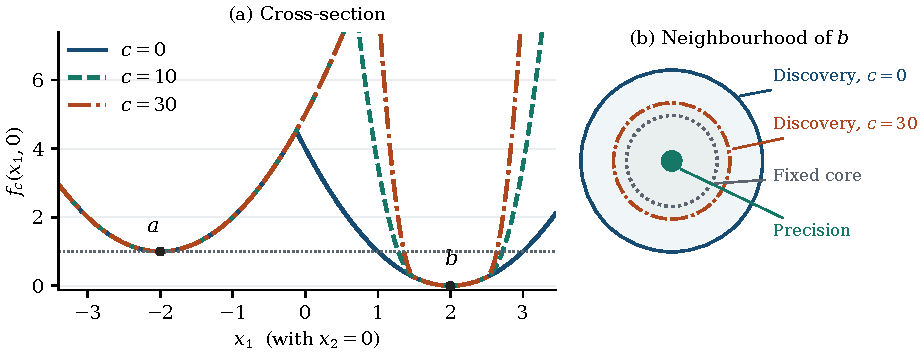
\includegraphics[width=.96\linewidth]{problem_geometry.pdf}
 \caption{Objective cross-section at \(x_2=0\) and target sets around \(b\). The discovery radius depends on \(c\). The fixed core and precision circle are unchanged and have radii \(0.5\) and \(0.1\), respectively.}
 \label{fig:geometry}
\end{figure}

Every main comparison uses \(T=50\) objective evaluations. In our experiments, unless otherwise stated, BO-EI uses four initial random evaluations, EI offset \(\xi=0\) and a GP noise parameter of \(10^{-10}\) for numerical stability. TuRBO-1 uses four initial design evaluations per start, batch size one and 50 GP training steps. CMA-ES uses a uniformly sampled initial mean on \([0,1]^2\), the default \texttt{pycma} population size, and initial step size \(\sigma_0=0.25\), corresponding to 2 units in the original coordinates. The implementation restarts if CMA-ES terminates before the budget is exhausted. Uniform random search draws independently from \(\mathcal X\).

Let \(F_t=\min_{1\leq i\leq t}f_c(x_i)\). Since \(f_c(b)=0\), \(F_t\) is the simple regret, ie. the difference between the found minimum and the true global minimum. We report empirical attainment of discovery, core entry and precision, corresponding to thresholds \(1\), \(0.25\) and \(10^{-2}\), together with terminal regret and first hitting times \cite{coco}. A missed target has hitting time \(+\infty\) by default. 






\section{Experiment 1. Baseline performance across penalties}
\label{sec:exp1}
We compare four methods at \(c\in\{0,3,10,30\}\), using ten seeds per method and penalty, for 160 runs in total. Table~\ref{tab:exp1} shows that the relative performance depends on the target. At \(c=0\), each adaptive method discovers B in nine runs, but BO-EI and TuRBO-1 attain precision in all nine, compared with two CMA-ES runs. As the penalty increases, discovery becomes less frequent for the BO variants. At \(c=10\), both attain discovery and precision twice, whereas CMA-ES discovers B seven times but reaches precision only twice. Such observation suggests that while CMA-ES is capable of discovering the optimum basin in multiple instances, it is less able to refine to the global minimum solution; BO and its variants have the opposite problem, being able to refine to a minimum solution but unable to discover the optimum basin.

\begin{table}[!htb]
 \centering
 \caption{Discovery / precision counts after 50 evaluations, out of ten runs per data point.}
 \label{tab:exp1}
 \begin{tabular}{rcccc}
 \toprule
 \(c\) & BO-EI & TuRBO-1 & CMA-ES & Uniform random\\
 \midrule
 0  & 9/9 & 9/9 & 9/2 & 10/1\\
 3  & 5/5 & 5/5 & 9/2 & 10/1\\
 10 & 2/2 & 2/2 & 7/2 & 9/1\\
 30 & 1/1 & 1/0 & 5/0 & 8/1\\
 \bottomrule
 \end{tabular}
\end{table}

Uniform random search has the highest observed discovery count at every penalty, but attains precision only once in each setting. We can derive that for \(T\) independent uniform evaluations,
\begin{equation}
\label{eq:uniform}
 \Pr(D_T)=
 1-\left(1-\frac{\pi\rho_c^2}{64}\right)^T,
 \qquad
 \Pr(P_T)=
 1-\left(1-\frac{\pi(0.1)^2}{64}\right)^T.
\end{equation}
where $D_T$ and $P_T$ denotes the event of already attaining discovery and precision by the $t^{th}$ evaluation, respectively. At \(T=50\), the precision probability is only about \(2.43\%\). Broad coverage can therefore produce frequent discoveries while remaining inefficient for precision. 

\begin{figure}[!htb]
 \centering
 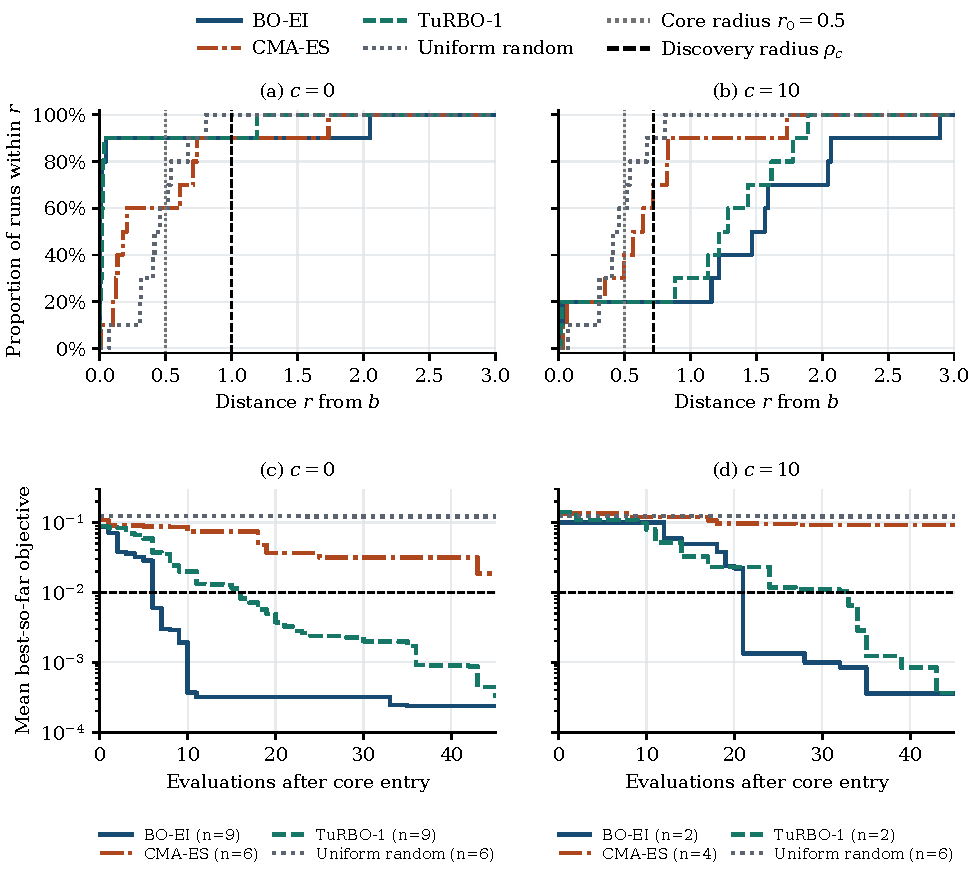
\includegraphics[width=.82\linewidth]{experiment1_c0_c10.pdf}
 \caption{Closest approach to \(b\) (top) and best-so-far values
 after first core entry (bottom), at \(c=0\) and \(c=10\).
 Only core-entering runs appear below. Crosses mark the final
 available evaluations; the dashed horizontal line is the
 precision threshold.}
 \label{fig:experiment1_diagnostics}
\end{figure}

Figure~\ref{fig:experiment1_diagnostics} illustrates such point. At \(c=10\), CMA-ES samples within distance 1 of \(b\) in nine runs, compared with two for BO-EI and three for TuRBO-1. Because this neighbourhood has fixed size, the difference cannot be explained solely by the shrinking discovery threshold as $c$ increases. CMA-ES enters the fixed core in four runs, compared with two for each BO variant, but all three attain precision twice. At \(c=0\), both BO variants attain precision in all nine core-entering runs, compared with two of six for CMA-ES.

These observations suggest a discovery bottleneck for the BO variants and less reliable refinement for default CMA-ES. We next test whether changing global coverage or sampling concentration alters the corresponding outcome. 
\section{Experiment 2. Within-method interventions}\label{sec:exp2}


\subsection{BO-EI recovery after an early miss}
\label{sec:bo_recovery}
For a GP posterior \(Y(x)\mid\mathcal D_t\sim\mathcal N(\mu_t(x),s_t^2(x))\), expected improvement with offset \(\xi\geq0\) is
\begin{equation}
\label{eq:ei}
 \EI_\xi(x)
 =\mathbb E[(F_t-\xi-Y(x))_+]
 =\delta_t(x)\Phi(z_t(x))+s_t(x)\phi(z_t(x)),
\end{equation}
where \(F_t\) is the best observed objective value,
\(\delta_t(x)=F_t-\xi-\mu_t(x)\),
\(z_t(x)=\delta_t(x)/s_t(x)\), and \(\Phi,\phi\) are the standard normal distribution and density. When \(s_t(x)=0\), EI equals \((\delta_t(x))_+\).

The offset \(\xi\) determines how much improvement is required before an outcome contributes positively to the acquisition. With \(\xi=0\), any improvement over \(F_t\) contributes. With \(\xi>0\), an outcome must improve on \(F_t\) by more than \(\xi\). Near an already explored local minimum, the posterior may predict only small further improvements with little uncertainty. Increasing \(\xi\) makes these evaluations less attractive. Less explored locations with greater posterior uncertainty may still offer a substantial chance of exceeding the larger improvement threshold, making them relatively more attractive.

As derived in \eqref{eq:uniform}, by sampling points via a uniform distribution on the space (we hereby refer this as 'uniform probes'), we have probability \(\pi\rho_c^2/64\) of hitting the discovery circle independently of the posterior. This motivates comparing a change to the acquisition offset with an explicit allocation of evaluations to global sampling.

At each of \(c=10,30\), 50 seeds first run standard BO-EI for 12 evaluations. For evaluations that do not discover the better basin, we copy the historical trajectories into four continuations: standard EI; EI with \(\xi=0.5\); standard EI with ten uniform probes; and the combination. Probes replace EI proposals at evaluations \(13,16,\ldots,40\), with the same probe locations used by both probe variants within a seed. All observations update the GP, and evaluations 41-50 use standard EI in every variant. The comparison between methods therefore measures recovery conditional on an early miss, within the same total budget.

\begin{table}[!htb]
 \centering
 \caption{Discovery / precision counts at evaluation 50 among
 histories with \(F_{12}\geq1\).}
 \label{tab:bo}
 \begin{tabular}{lcc}
 \toprule
 Continuation & \(c=10\), \(n=39\) & \(c=30\), \(n=42\)\\
 \midrule
 Standard BO-EI       & 8/7   & 1/1\\
 \(\xi=0.5\)          & 14/14 & 8/7\\
 Uniform probes      & 27/23 & 21/14\\
 \(\xi=0.5\) + probes & 31/28 & 22/14\\
 \bottomrule
 \end{tabular}
\end{table}

Uniform probes increase discovery by 48.7 percentage points at \(c=10\) (95\% CI \([17.4,69.6]\)) and 47.6 points at \(c=30\) (\([20.2,65.6]\)). Precision also increases, by 41.0 and 31.0 points, with intervals \([13.1,60.1]\) and \([3.7,51.7]\). Increasing \(\xi\) alone gives smaller observed gains, whose intervals include zero. The additional benefit of increasing \(\xi\) is more significant when $c=10$. As the global basin becomes harder to find, the benefits become less significant.

The trajectories support the proposed coverage explanation. During evaluations 13--40, probes increase the mean number of newly visited unit grid cells from 5.0 to 13.6 at \(c=10\) and from 3.4 to 12.8 at \(c=30\). The fraction of evaluations within distance 1 of \(a\) decreases from \(73\%\) to \(36\%\) and from \(85\%\) to \(44\%\). Of the discoveries under standard EI with probes, 9 occur at probes and 18 at EI proposals for \(c=10\); the corresponding counts are 11 and 10 for \(c=30\). Thus the policy can help through both directly reaching the basin or subsequent model-guided evaluations from the discovery-favouring method. 

\begin{figure}[!htb]
 \centering
 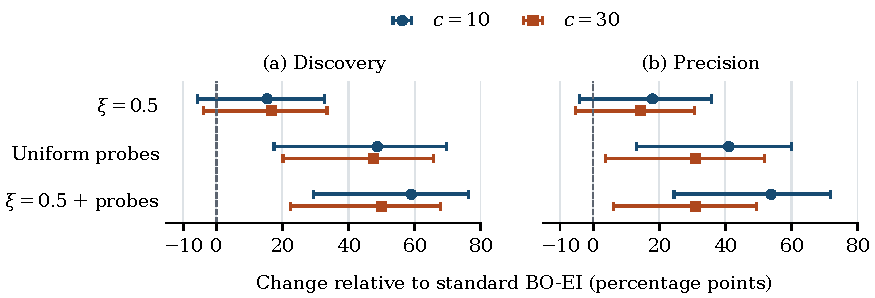
\includegraphics[width=.90\linewidth]{bo_paired_effects.pdf}
 \caption{Paired differences in target-attainment proportions relative to standard BO-EI. Bars show conservative 95\% confidence intervals for individual contrasts.}
 \label{fig:boeffects}
\end{figure}


\subsection{Trust-region contraction and restarts in TuRBO-1}
TuRBO-1 uses Thompson sampling from a local GP posterior within an adaptive trust region centred on the incumbent. The trust region contracts after a specified number of consecutive unsuccessful iterations and restarts when its length falls below a minimum threshold. To investigate whether premature concentration around the inferior basin limits discovery, we vary the normalised initial trust-region length \(L_0\) and failure tolerance \(k_{\rm fail}\). The six variants share four initial design points within each seed, with all 50 seeds per penalty included in the comparison. The configurations differ from the first model-guided proposal onward.

\begin{table}[!htb]
 \centering
 \caption{TuRBO-1 outcomes after 50 evaluations. Each cell reports discovery count / precision count / count of runs with at least one restart, out of 50 runs.}
 \label{tab:turbo}
 \begin{tabular}{lcccc}
 \toprule
 Variant & \(L_0\) & \(k_{\rm fail}\) & \(c=10\) & \(c=30\)\\
 \midrule
 Default               & 0.8 & 4  & \(12/9/30\)  & \(5/4/29\)\\
 Small region          & 0.4 & 4  & \(20/10/45\) & \(11/5/41\)\\
 Large region          & 1.6 & 4  & \(12/10/26\) & \(6/5/24\)\\
 Fast contraction      & 0.8 & 2  & \(19/13/50\) & \(14/9/50\)\\
 Slow contraction      & 0.8 & 8  & \(10/9/0\)   & \(4/3/0\)\\
 Very slow contraction & 0.8 & 12 & \(11/9/0\)   & \(4/3/0\)\\
 \bottomrule
 \end{tabular}
\end{table}

Smaller initial regions and faster contraction improve discovery under the fixed evaluation budget (Table~\ref{tab:turbo}). At \(c=30\), fast contraction increases discovery from 5/50 to 14/50 and precision from 4/50 to 9/50. It also advances the median first restart from evaluation 44 to 28, with all 50 runs restarting compared with 29 under the default configuration. In contrast, both slower-contraction variants record no restarts and only 4/50 discoveries.

The evaluation histories provide further insight into how restarts contribute to discovery. At \(c=30\), nine of the 14 successful fast-contraction runs first discover the better basin after restarting, including seven during the fresh four-point initial design and two during subsequent local search. This suggests that restarts can facilitate discovery both directly through renewed global sampling and indirectly by enabling local search in a new region.

The smaller initial-region variant also improves discovery to 11/50 at \(c=30\), although its median first restart occurs at evaluation 42, only slightly earlier than the default. Of its 11 discoveries, two occur during restart initialisation and four during subsequent local search. Thus, restart timing alone does not fully explain the observed differences; changes in local search trajectories may also contribute.

Overall, these results suggest that abandoning an unpromising trust region and restoring broader exploration can improve TuRBO-1's discovery performance on the two-basin objective. However, the interventions also change the proposals before restarting, so the observed improvements cannot be attributed exclusively to restarts.

\subsection{Effects of population size, parent count, and mean updates
on CMA-ES discovery and precision}

Experiment~1 showed that CMA-ES can discover the better basin without
reaching the precision target. We examine how population size
\(\lambda\), the number of selected parents \(\mu\), and the size of
the mean update affect discovery, precision, and settling near \(b\).
We study settling speed at \(c=3\) and compare discovery and precision
at \(c=30\). In the comparisons reported here, we initialise the search
mean at \((1.8,0)\), \((1.6,0)\), or \((1.4,0)\).
Each configuration uses the same 20 seeds at each starting location,
giving 60 matched seed--offset combinations. We record discovery and
precision for the same runs at 50 and 200 objective evaluations.

We first vary population size and settling speed.
At \(c=3\), we compare CMA-ES populations of 6 and 12, with
\(\mu=\lambda/2\). We pair runs by seed and starting location.
To measure how quickly the search concentrates around \(b\), we use
the root-mean-square (RMS) distance of the sampling distribution to \(b\),
\[
D_b=\sqrt{\|m-b\|_2^2+\operatorname{tr}(\Sigma)},
\]
where \(m\) is the search mean and \(\Sigma\) is the sampling covariance,
both expressed on the original domain. The settling evaluation is the
first evaluation from which \(D_b\) stays below \(0.4\) through
evaluation 200. Among the 37 matched pairs in which both configurations
settled near \(b\), the population of 6 settled sooner in 30 pairs,
tied in four, and settled later in three
(Figure~\ref{fig:cmaes-results}, top row, panel (a)).
Across all 60 runs per configuration, the median RMS distance to \(b\)
generally decreased faster and remained lower for \(\lambda=6\) over
most of the evaluation budget
(Figure~\ref{fig:cmaes-results}, top row, panel (b)).
At evaluation 50, it was \(0.88\) for
\(\lambda=6\) and \(1.36\) for \(\lambda=12\). Both medians were close
to zero by evaluation 200, indicating that the smaller population
typically concentrated around \(b\) sooner. Across all runs,
\(\lambda=12\) finished near \(b\) more often (52 versus 42 runs).
Overall, the smaller population tended to concentrate around \(b\)
sooner, while the larger population finished near \(b\) in more runs.

We then vary parent count at a fixed population size.
With \(\lambda=12\) fixed, the bottom-left plot in
Figure~\ref{fig:cmaes-results} shows that discovery (\(f<1\))
increased as more parents were selected. Precision (\(f<0.01\)) and
the share of runs whose sampling distributions finished near \(b\)
generally decreased, with a slight recovery at the largest parent
count. Since each setting evaluated the same number of candidates
per generation, the difference concerns how those candidates were
used to update the search. For runs starting near \(b\), selecting
more parents favoured discovery, while selecting fewer was associated
with both greater concentration near \(b\) and more precise solutions.

We also halve the mean update.
At \(c=30\), starting near \(b\), the halved mean update outperformed
the standard update on both discovery and precision. In the left plot
of the bottom-right panel of Figure~\ref{fig:cmaes-results},
the discovery curve (\(f<1\)) rises faster and stays above the
standard-update curve once they separate. In the right plot, the
precision curve (\(f<0.01\)) also pulls ahead, and its lead grows as
more evaluations are used. By 200 evaluations, the halved update
achieved discovery in 53 of 60 runs, compared with 44 under the
standard update, and reached precision in 33 runs, compared with 16.
The advantage therefore extended from finding the better basin to
reaching the stricter precision target.

\begin{figure}[!htbp]
\centering
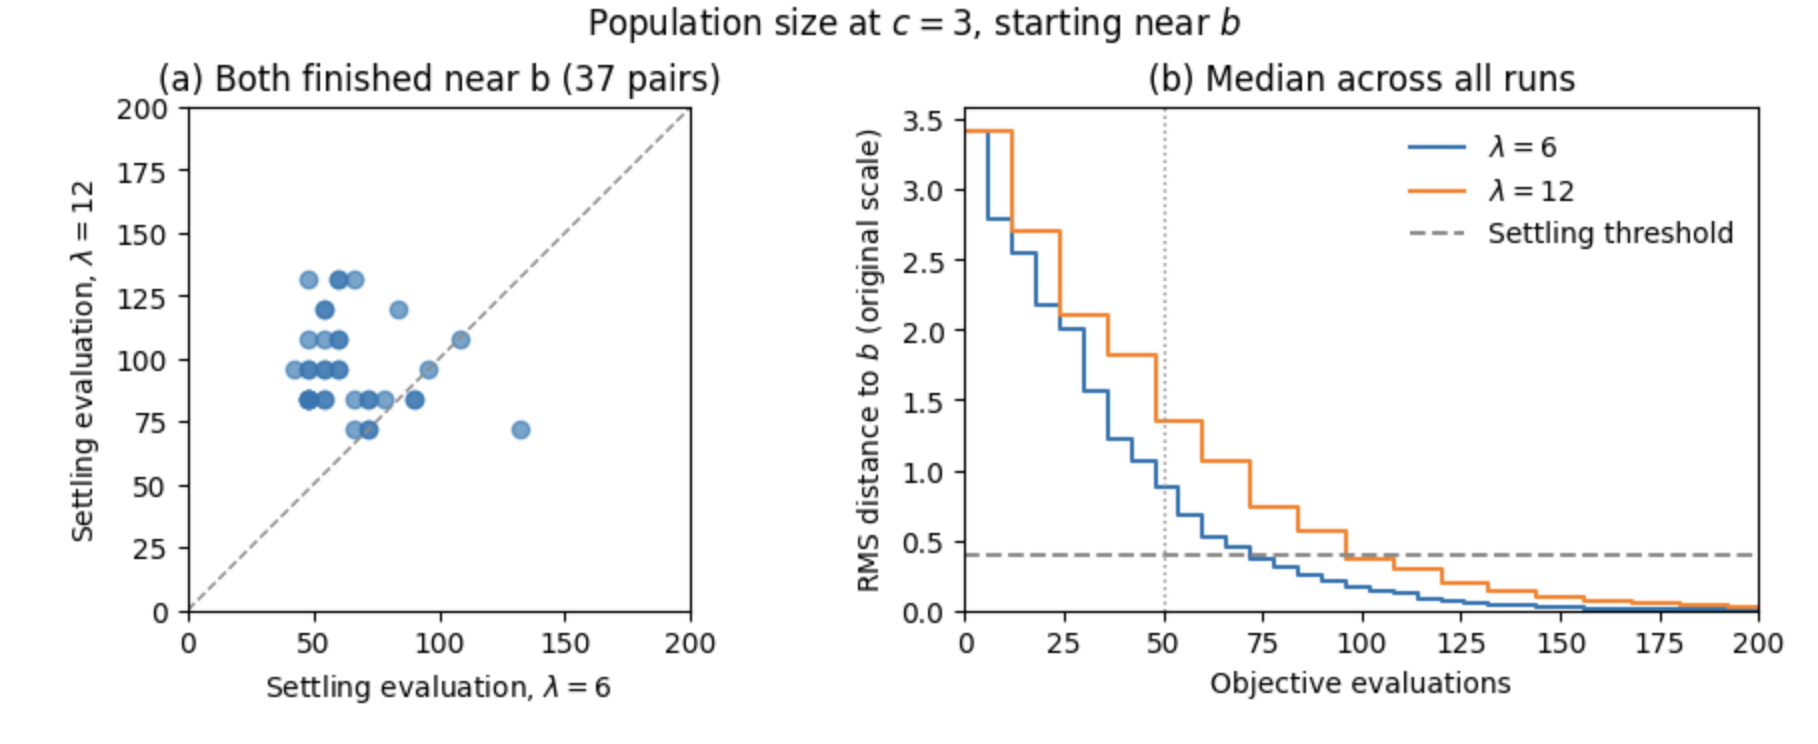
\includegraphics[width=0.78\linewidth]{1.png}\par
\smallskip
\noindent
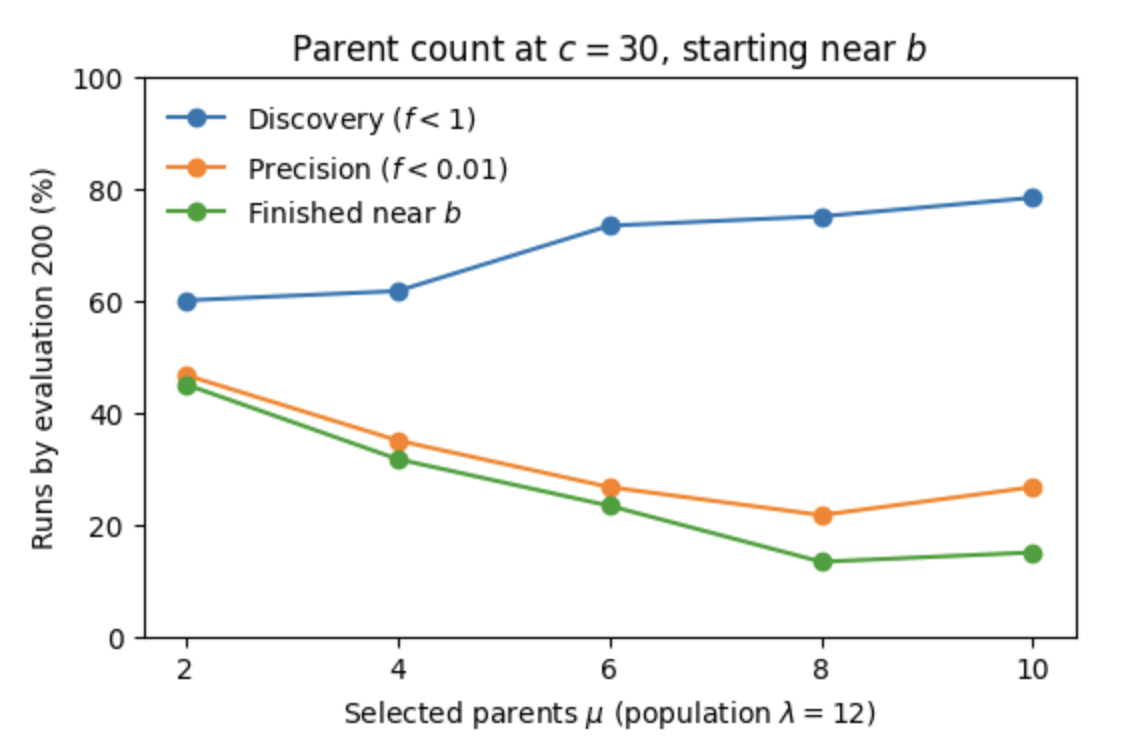
\includegraphics[width=0.36\linewidth]{2.png}\hfill
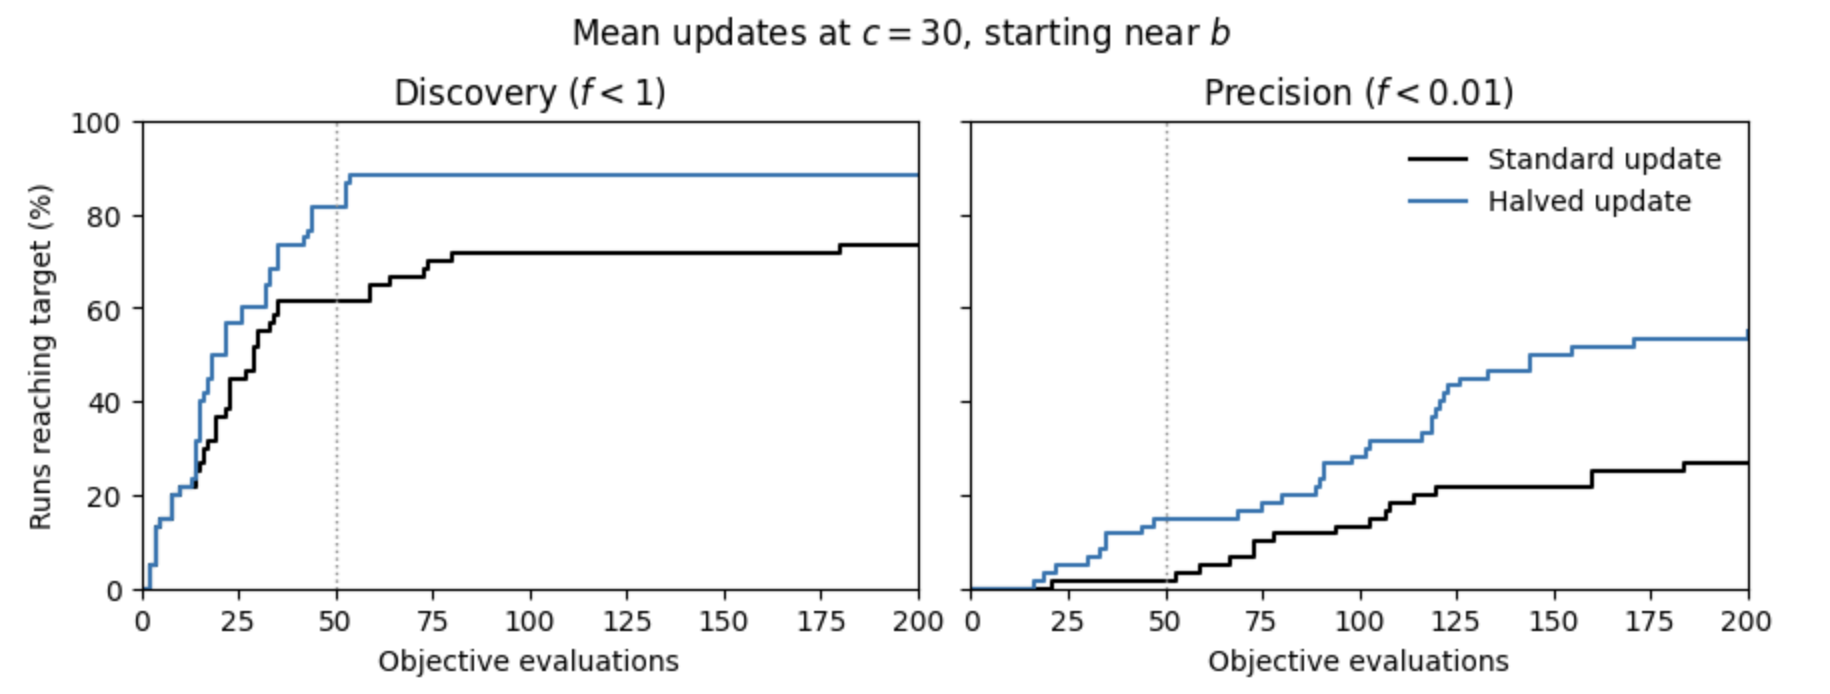
\includegraphics[width=0.61\linewidth]{3.png}\par
\caption{CMA-ES runs starting near \(b\).
The top row shows paired settling evaluations (a) and median RMS
distance to \(b\) (b) for populations of 6 and 12 at \(c=3\).
The bottom-left plot shows outcomes at evaluation 200 across parent
counts at \(c=30\) and \(\lambda=12\).
The bottom-right panel shows cumulative discovery (left) and precision
(right) for the standard and halved mean updates at \(c=30\).}
\label{fig:cmaes-results}
\end{figure}

At \(c=3\), the smaller population usually settled sooner among
pairs where both settled near \(b\), while the larger population
finished near \(b\) more often overall. At \(c=30\), the population
and parent-count comparisons
show a trade-off by 200 evaluations. The smaller configurations
yielded fewer discoveries and more precision hits. Halving the mean
update improved both outcomes when CMA-ES started near \(b\), and
the search mean ended closer to \(b\). Experiment~3 builds on this
finding by comparing BO and CMA-ES under initial designs near \(A\)
and \(B\) to test how starting information affects discovery and
refinement.





\section{Experiment 3. Initial information and tradeoff of exploration}\label{sec:controlled}
Experiment 2 shows how changing search policies can affect discovery and refinement. We now test how their value depends on the information available at the start. The prediction is that global probes should be most useful when observations support the inferior basin A, whereas local concentration should be most useful when they already identify B.

At \(c=30\), each of 50 seeds has eight common background points outside the unit disks around both minima. Four additional points lie at radii \(0.35,0.39,0.43,0.47\) around either A or B, using the same randomly rotated directions in both designs. The initial best values are therefore \(1.1225\) near A and \(0.1225\) near B. All 12 observations count towards the budget, leaving 38 evaluations. Every near-B design has already attained discovery and core entry, but none has attained precision.

Standard BO-EI and BO-EI with probes fit to the same 12 observations and differ only by the ten-probe, as given Section~\ref{sec:bo_recovery}. Both CMA-ES variants initialise their means at the best observed point and use the same default population size and adaptation rules. They differ only in normalised initial step size: \(\sigma_0=0.25\) or \(0.05\), where bigger step size encourages exploration. Note that both variants subsequently adapt their step sizes. 

\begin{table}[!htb]
 \centering
 \caption{Experiment 3: attainment counts out of 50 runs}
 \label{tab:controlled}
 \begin{tabular}{lrrrr}
 \toprule
 & \multicolumn{3}{c}{Initial design near A} & Near B\\
 \cmidrule(lr){2-4}\cmidrule(l){5-5}
 Method & Discovery & Refinement near A & Precision & Precision\\
 \midrule
 Standard BO-EI            & 1  & 50 & 0 & 42\\
 BO-EI + probes            & 16 & 48 & 5 & 36\\
 CMA-ES, \(\sigma_0=0.25\) & 5 & 7 & 0 & 4\\
 CMA-ES, \(\sigma_0=0.05\) & 0 & 46 & 0 & 46\\
 \bottomrule
 \end{tabular}
\end{table}

Near A, probes increase BO-EI discovery from \(1/50\) to \(16/50\), a paired difference of 30 percentage points (95\% CI \([8.1,46.6]\)); five probe runs also attain precision (Table~\ref{tab:controlled}). Standard BO-EI refines near A in all 50 runs, showing that accurate local optimisation can coexist with failure to discover the better
region. 

Near B, standard BO-EI attains precision in \(42/50\) runs, compared with \(36/50\) with probes. Median terminal regret increases from \(0.00190\) to \(0.00495\). This illustrates the exploration-exploitation tradeoff, where probes consume evaluations that could otherwise refine a known promising region.

In the near-B experiment, reducing the initial CMA-ES scale raises precision from \(4/50\) to \(46/50\), a paired increase of 84 percentage points (95\% CI \([60.6,93.7]\)). The fraction of continuation evaluations inside the radius-0.5 core increases from \(5.9\%\) to \(75.6\%\), or approximately 2.3 versus 28.7 of the 38 available evaluations per run. At the larger scale, median terminal regret remains at the initial value of \(0.1225\), despite the supplied point already lying in the core. This supports the explanation that access to a good point is insufficient when subsequent sampling is poorly concentrated around it.

Near A, the same reduction increases refinement around the inferior minimiser from \(7/50\) to \(46/50\), while discovery changes from
\(5/50\) to \(0/50\). Smaller scale therefore improves local refinement at either starting location, but only refinement near B achieves the global precision target. These results explain why the scale and adaptation changes in Experiment 2 for CMA do not have a universal benefit: their consequences depend on which region receives more evaluations.

\begin{figure}[!htb]
 \centering
 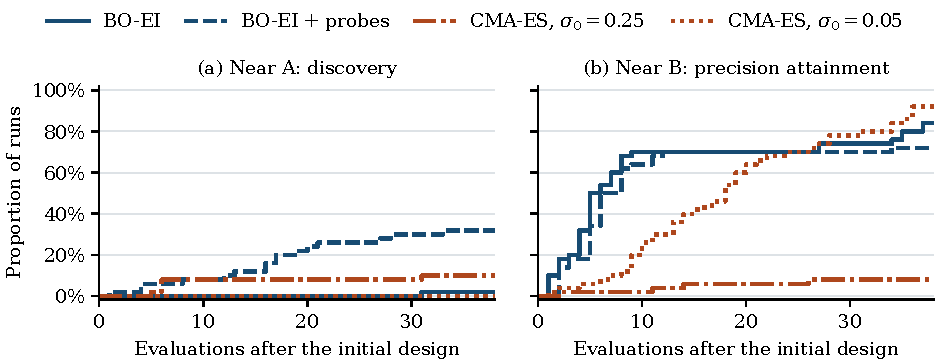
\includegraphics[width=.84\linewidth]{controlled_hits.pdf}
 \caption{Target attainment after the 12-evaluation initial design in Experiment 3. The near-A panel measures discovery, and the near-B panel measures precision.}
 \label{fig:controlled}
\end{figure}

Figure~\ref{fig:controlled} illustrates clearly the tradeoff of methods that favour exploration. Note that for methods such that BO with probes or CMA with larger $\sigma_0$ which prefer exploration, the methods often report a better ability to find the global minimum, but taken at a cost that when it reaches the optimum basin, they are less likely to find the actual minimum. Taken with Experiment 2, the evidence supports a dependence of the performance of methods on search location.
\section{Discussion}\label{sec:discussion}

Precision attainment requires both discovering B and reaching the tighter target after discovery. Experiment~1 considers a general run of the compared methods. At \(c=0\), all three adaptive methods have the same discovery count, yet BO-EI and TuRBO-1 convert more discoveries into precise solutions than CMA-ES. As \(c\) increases, both BO variants visit a fixed neighbourhood of \(b\) less frequently. The decline in discovery therefore reflects changed sampling behaviour and inability of the BO algorithm to find the smaller basin.

For BO-EI, a smooth Gaussian process may extrapolate high values from the outer part of B across its unobserved core, leaving higher EI near \(a\).  In Experiment~2, uniform probes imporve coverage directly, whereas increasing \(\xi\) still ranks points using the fitted posterior. The probe policy also changes what the GP learns, so its measured recovery benefit includes subsequent EI proposals. Experiment~3 illustrates how the role of probes changes with the initial information. Once B is observed, the ten probes replace evaluations that EI could devote to refinement, which is reflected in the decrease of precision decrease.

For TuRBO-1, discoveries during restarted designs support the role of renewed global coverage. Faster contraction also changes proposals before a restart and can reduce the time spent refining the current incumbent. 

In CMA-ES, a single candidate can discover basin B and immediately improve the incumbent, while the search distribution updates once per generation. Larger populations draw more candidates per generation and allow fewer updates under a fixed evaluation budget. In Experiment 2, among matched runs that both settled near B, the smaller population generally settled sooner. Across all runs, the larger population finished near B more often. Halving the mean update also improved discovery and precision from near B, consistent with keeping the search centred closer to the global minimiser.  Experiment~3 tests the dispersion explanation more directly. From the same mean near B, a smaller step size concentrates more evaluations in the core and substantially improves precision. From near A, the same concentration favours refinement around the inferior minimiser. The gain from slower mean adaptation near B in Experiment~2 is also consistent with retaining a promising search centre.

\section{Conclusion}\label{sec:conclusion}
Under a budget of 50 evaluations, discovery and precision reveal different weaknesses in the tested methods. Global probes improve BO-EI recovery after an early miss, and TuRBO-1 results support renewed global sampling through restarts. CMA-ES attains higher precision with a smaller initial step size,
fewer selected parents, or a halved mean update when its mean is
already near the global minimiser. A smaller population also tends
to concentrate the search there sooner, suggesting faster local
refinement. When the mean starts near the inferior minimiser,
a smaller initial step size can reinforce refinement around that
solution. On this benchmark, the benefits of exploration and concentration depend on instances, search location, target accuracy and the domain of evaluation.

% Beckham

\begingroup
\small
\RenewDocumentCommand{\chapter}{s o m}{\section*{#3}}
\renewcommand{\bibname}{References}
\begin{thebibliography}{9}\setlength{\itemsep}{2pt}
\bibitem{frazier}
P.~I. Frazier. A tutorial on Bayesian optimization.
\emph{arXiv:1807.02811}, 2018.
\href{https://arxiv.org/abs/1807.02811}{arXiv}.
\bibitem{eriksson}
D. Eriksson, M. Pearce, J.~R. Gardner, R.~D. Turner, and M. Poloczek.
Scalable global optimization via local Bayesian optimization.
\emph{Advances in Neural Information Processing Systems}, 32, 2019.
\href{https://arxiv.org/abs/1910.01739}{arXiv}.
\bibitem{hansen}
N. Hansen. The CMA evolution strategy: A tutorial.
\emph{arXiv:1604.00772}, 2016, revised 2023.
\href{https://arxiv.org/abs/1604.00772}{arXiv}.
\bibitem{coco}
N. Hansen, A. Auger, R. Ros, O. Mersmann, T. Tušar, and D. Brockhoff.
COCO: A platform for comparing continuous optimizers in a black-box setting.
\emph{Optimization Methods and Software}, 36(1), 114--144, 2021.
\href{https://doi.org/10.1080/10556788.2020.1808977}{DOI}.
\bibitem{repo}
DSA4212 Group 1 Implementation.
\href{\repotree}{GitHub repository}.
\end{thebibliography}
\endgroup
\end{document}
